\section{Reversible jump MCMC for tree updates}\label{appendix:comp_details}

This section provides technical details on the reversible jump Metropolis--Hastings updates used to sample tree structures and their associated parameters in our model.
We update the tree structure $\mathcal{T}$ and step heights $\mathcal{H}$ jointly using the reversible jump framework \citep{ReversibleJump}.
We denote the current tree by $(\mathcal{T}, \mathcal{H})$ and the proposed tree by $(\mathcal{T}*, \mathcal{H}*)$.
We consider three reversible jump moves: \texttt{GROW}, \texttt{PRUNE}, and \texttt{CHANGE}, selected with fixed prior probabilities $P_\texttt{GROW}$, $P_\texttt{PRUNE}$, and $P_\texttt{CHANGE}$.
These moves enable exploration of the posterior by proposing local modifications to $(\mathcal{T}, \mathcal{H})$.

This section is organised as follows:
\begin{itemize}
    \item We begin with a brief recap of the model setup and prior specification.
    \item We then provide a detailed derivation of the acceptance ratio for the \texttt{GROW} move, which involves a change in model dimensionality.
    \item Finally, we explain how the acceptance ratios for the \texttt{PRUNE} and \texttt{CHANGE} moves follow from similar principles.
\end{itemize}

An overview of the steps involved in a single-tree reversible jump update is given in Algorithm~2 \citep{main_article}. 

\subsection{Recap of model setup and prior specification}

We model the log-transformed survival times as a noisy sum of regression trees:
\begin{equation}\label{model_appendix}
\log T_i = \sum_{j=1}^m g(X_i; \mathcal{T}_j, \mathcal{H}_j) + \varepsilon_i, \quad \varepsilon_i \sim \mathcal{N}(0, \sigma^2),
\end{equation}
where $m$ denotes the number of trees, $\mathcal{T}_j$ is the tree structure, and $\mathcal{H}_j$ is the set of step height parameters for the $j$-th tree.

We place independent priors on each pair $(\mathcal{T}_j, \mathcal{H}_j)$. The prior on the tree structure $\mathcal{T}$, originally proposed by \citet{BayesianCART}, is defined as follows:
\begin{enumerate}
    \item Start with a single root node.
    \item A leaf node at depth $d$ is split with probability:
    \begin{equation}\label{tree_prior}
        \rho_d := \frac{a}{(1 + d)^b},
    \end{equation}
    where $a \in (0, 1)$ and $b \geq 0$ are hyperparameters.
    \item The splitting variable is chosen uniformly at random from the available predictors.
    \item The split point is chosen uniformly from the observed values of the selected variable.
\end{enumerate}

The prior on the step height parameters $\mathcal{H}$, including any auxiliary parameters (e.g., local shrinkage parameters), is denoted by $p_\mathcal{H}(\mathcal{H} \mid \mathcal{T})$. Details can be found in Section~3.2 \citep{main_article}.

Posterior updates for $(\mathcal{T}, \mathcal{H})$ are based on the residuals derived from the current model fit. For the $j$-th tree, these are given by:
\begin{equation}\label{residuals_appendix}
\mathcal{R}_j := \log T^o - \sum_{J \ne j} g(X; \mathcal{T}_J, \mathcal{H}_J),
\end{equation}
where $T^o$ denotes the observed or imputed survival times after data augmentation.






\subsection{The \texttt{GROW} move}

When a \texttt{GROW} move is selected with probability $P_{\texttt{GROW}}$, the algorithm proposes to expand the current tree by splitting one of its terminal nodes (a leaf) into two new child nodes. 
This move increases the dimension of the parameter space and therefore requires a reversible jump step to ensure correct posterior exploration. 
The split is performed by selecting a valid splitting rule---that is, a covariate and a split point---which partitions the observations within the chosen parent node.

Consider a tree with three terminal nodes and corresponding step heights ${h_1, h_2, h_3}$, as illustrated on the left side of Figure~\ref{fig:GROWN_tree}. 
Suppose we select the third leaf node (associated with $h_3$) for a \texttt{GROW} move. 
A splitting rule is applied to this node, yielding two new child nodes. 
These new regions inherit a subset of the observations from the parent node, based on the splitting rule, and are each assigned their own proposed step heights, denoted $h_3'$ and $h_4'$. 
The resulting tree, shown on the right side of Figure~\ref{fig:GROWN_tree}, now contains four leaf nodes.

\input tikz_GROW_trees


The same transition can be viewed in the covariate space in Figure~\ref{fig:partition_grow}.
The left square represents the region before the split (corresponding to $h_3$) and the right square shows the refined partition into $h_3'$ and $h_4'$. 
This diagram offers geometric intuition for how the \texttt{GROW} move expands the parameter space by refining the partition of the covariate domain.

\input tikz_GROW_domain


Let $\texttt{P}$ denote the parent node being split, which has associated parameters $(h_\texttt{P}, \theta_\texttt{P})$, where $\theta_\texttt{P}$ represents local auxiliary parameters. 
For example, under the horseshoe prior with auxiliary variables (see Equation~12, \citealp{main_article}), we have $\theta_\texttt{P} = (\lambda_\texttt{P}^2, \nu_\texttt{P})$. 
The \texttt{GROW} move proposes two new sets of parameters for the child nodes: $(h_\texttt{L}, \theta_\texttt{L})$ and $(h_\texttt{R}, \theta_\texttt{R})$, where $\texttt{L}$ and $\texttt{R}$ denote the left and right child nodes as determined by the splitting rule. 

These proposed values are drawn from pseudo Gibbs proposal distributions, as described in Section~4.2 \citep{main_article}. 
The proposals are informed by the current parameters within the tree and the observed data: new values for the step heights and local parameters are generated from conditional distributions influenced by those of the parent node. 
While this resembles a Gibbs sampler, it is not a true one — the parent node’s parameters cannot be directly sampled since the node is replaced by two new children. 
This is not problematic as the Metropolis-Hastings acceptance step guarantees that the Markov chain targets the correct posterior, thereby ensuring convergence to the stationary distribution. 
The overarching goal is to construct proposals that are both informed and efficient.

We now derive the reversible acceptance ratio $r_\texttt{GROW}$ for a \texttt{GROW} move. 
Note that the acceptance probability is given by $\min\{1, r_\texttt{GROW}\}$. 
The general framework for deriving the reversible jump acceptance ratio is outlined by \citet{ReversibleJump}. 
Following this approach, the acceptance ratio builds on the Metropolis--Hastings formulation, as applied to tree-based models by \citet{BARToriginal}, and incorporates both the proposal densities of the step heights and the determinant of the Jacobian associated with the parameter transformation. 
A comprehensive overview of how to derive acceptance ratios for non-reversible updates in standard BART is provided by \citet{Kapelner2016}.

We must satisfy the dimension-matching condition introduced by \citet{ReversibleJump} to perform a valid reversible jump move. 
Suppose we split a leaf node with associated parameters $(h_\texttt{P}, \theta_\texttt{P})$ into two child nodes with new parameters $(h_\texttt{L}, \theta_\texttt{L})$ and $(h_\texttt{R}, \theta_\texttt{R})$. 
We can interpret the parent node as having already been split, but with the child nodes initially inheriting the same values as the parent. 
This construction yields the same conditional posterior distribution and facilitates a reversible proposal structure. 
A schematic overview of this matching is depicted in Figure~\ref{fig:dim_match}. 
The Jacobian of the transformation is equal to one because the new parameters are randomly drawn using the pseudo Gibbs proposal mechanism.



\input tikz_dim_match

We derive the acceptance ratio $r_\texttt{GROW}$ for a \texttt{GROW} move. 
This ratio compares the probability of proposing and accepting a move to a larger tree versus reversing that move. 
It is given by:
\begin{equation}
    r_\texttt{GROW} = \frac{q\big((\T, \H) \to (\T_*, \H_*)\big)}{q\big((\T_*, \H_*) \to (\T, \H)\big)} \cdot \frac{p\big((\T, \H) \ | \ \mathcal{R}, \sigma^2\big)}{p\big((\T_*, \H_*) \ | \ \mathcal{R}, \sigma^2\big)},
\end{equation}
where $q(\cdot \to \cdot)$ denotes the transition probability between tree states, and $p(\cdot \mid \mathcal{R}, \sigma^2)$ is the conditional posterior distribution given the residuals and noise level.

By applying Bayes' rule to the posterior terms, we rewrite the ratio as:
\begin{equation}
\begin{split}
    r_\texttt{GROW} 
    &= \underbrace{\frac{q\big((\T, \H) \to (\T_*, \H_*)\big)}{q\big((\T_*, \H_*) \to (\T, \H)\big)}}_{\text{transition ratio}} 
    \cdot 
    \underbrace{\frac{\mathcal{L}\big(\mathcal{R} \mid \T, \H, \sigma^2\big)}{\mathcal{L}\big(\mathcal{R} \mid \T_*, \H_*, \sigma^2\big)}}_{\text{likelihood ratio}} 
    \cdot 
    \underbrace{\frac{p\big(\T, \H\big)}{p\big(\T_*, \H_*\big)}}_{\text{prior ratio}},
\end{split}
\end{equation}
where $\mathcal{L}$ is the likelihood of the residuals (see Equation~10, \citealp{main_article}), and $p(\T, \H)$ denotes the joint prior over tree structure $\T$ and step height parameters $\H$.


The likelihood only changes for observations in the node being split. For all other observations, the likelihood remains the same. As a result, the likelihood ratio simplifies to:
\begin{equation}
    \frac{\mathcal{L}\big(\mathcal{R} \mid \T, \H, \sigma^2\big)}{\mathcal{L}\big(\mathcal{R} \mid \T_*, \H_*, \sigma^2\big)} = \frac{\prod_{i \in \texttt{P}} \mathcal{N}(\mathcal{R}_i \mid h_\texttt{P}, \sigma^2)}{\prod_{i \in \texttt{L}} \mathcal{N}(\mathcal{R}_i \mid h_\texttt{L}, \sigma^2) \cdot \prod_{i \in \texttt{R}} \mathcal{N}(\mathcal{R}_i \mid h_\texttt{R}, \sigma^2)},
\end{equation}
where $\texttt{P}$ is the parent node being split, and $\texttt{L}$ and $\texttt{R}$ are the resulting left and right child nodes.
We write $i \in \texttt{L}$ to denote that observation $i$ falls into node $\texttt{L}$ under the tree partitioning.

The prior ratio decomposes into the ratio of the tree structure priors and the prior on the step heights:
\begin{equation}
\begin{split}
    \frac{p(\T, \H)}{p(\T_*, \H_*)} &= \frac{p_\mathcal{T}(\T)}{p_\mathcal{T}(\T_*)} \cdot \frac{p_\mathcal{H}(\H \mid \T)}{p_\mathcal{H}(\H_* \mid \T_*)} \\
    &= \frac{\rho_d(1-\rho_{d+1})^2}{1 - \rho_d} \cdot \frac{p(h_\texttt{P} \mid \theta_\texttt{P}) \, p(\theta_\texttt{P})}{p(h_\texttt{L} \mid \theta_\texttt{L}) \, p(\theta_\texttt{L}) \cdot p(h_\texttt{R} \mid \theta_\texttt{R}) \, p(\theta_\texttt{R})},
\end{split}
\end{equation}
where $d$ is the depth of the split node, and $\rho_d$ is the depth-dependent internal node probability from the tree prior (see Equation~\eqref{tree_prior}).

The transition ratio accounts for move probabilities, available node choices, and proposal densities:
\begin{equation}
    \frac{q\big((\T, \H) \to (\T_*, \H_*)\big)}{q\big((\T_*, \H_*) \to (\T, \H)\big)} 
    = \frac{P_\texttt{GROW}}{P_\texttt{PRUNE}} \cdot \frac{k^{-1}}{N_*^{-1}} \cdot \frac{q_\texttt{PRUNE}(h_\texttt{P}, \theta_\texttt{P})}{q_\texttt{GROW}(h_\texttt{L}, \theta_\texttt{L}) \cdot q_\texttt{GROW}(h_\texttt{R}, \theta_\texttt{R})},
\end{equation}
where $k$ is the number of leaf nodes in the current tree, $N_*$ is the number of eligible internal nodes (nog nodes) in the proposed tree, and $q$ refers to the proposal distributions.
We use the notation $q_\texttt{MOVE}$ to denote the proposal distribution used in each move, which is typically constructed as a pseudo Gibbs draw informed by the current state and residuals.


\subsection{The \texttt{PRUNE} and \texttt{CHANGE} moves}

In a \texttt{PRUNE} move, a \textit{nog} node (a parent node with exactly two children) is selected, and its children are removed. 
This corresponds to merging two adjacent subregions in the covariate space. 
The \texttt{PRUNE} move is the exact inverse of the \texttt{GROW} move. 
As a result, its reversible jump acceptance ratio $r_\texttt{PRUNE}$ is the reciprocal of the acceptance ratio for the corresponding \texttt{GROW} move:
\begin{equation}
    r_\texttt{PRUNE} = \frac{1}{r_\texttt{GROW}}.
\end{equation}

To propose parameters for the resulting leaf node, we must construct a reverse mapping from the child parameters. 
Several strategies are possible, such as averaging the child values or restoring the original parent values. 
We adopt the latter: the \texttt{PRUNE} move reverts to the parameter values of the parent node prior to the corresponding \texttt{GROW} move.

The \texttt{CHANGE} move modifies the splitting rule of an internal node while keeping the tree structure and parameter dimension fixed. 
Since the number of parameters remains unchanged, the reversible jump acceptance ratio $r_\texttt{CHANGE}$ includes a likelihood ratio, a proposal ratio, and a prior ratio for the step height parameters.

Suppose we propose new values $(h_{\texttt{L}*}, \theta_{\texttt{L}*})$ and $(h_{\texttt{R}*}, \theta_{\texttt{R}*})$ to replace the current parameters $(h_\texttt{L}, \theta_\texttt{L})$ and $(h_\texttt{R}, \theta_\texttt{R})$. The acceptance ratio becomes:
\begin{equation}
\begin{split}
    r_\texttt{CHANGE} 
    &= \frac{\prod_{i \in \texttt{L}} \mathcal{N}(\mathcal{R}_i \mid h_\texttt{L}, \sigma^2) \prod_{i \in \texttt{R}} \mathcal{N}(\mathcal{R}_i \mid h_\texttt{R}, \sigma^2)}{\prod_{i \in \texttt{L}*} \mathcal{N}(\mathcal{R}_i \mid h_{\texttt{L}*}, \sigma^2) \prod_{i \in \texttt{R}*} \mathcal{N}(\mathcal{R}_i \mid h_{\texttt{R}*}, \sigma^2)} \\
    &\quad \times \frac{q_\texttt{CHANGE}(h_{\texttt{L}*}, \theta_{\texttt{L}*}) \, q_\texttt{CHANGE}(h_{\texttt{R}*}, \theta_{\texttt{R}*})}{q_\texttt{CHANGE}(h_\texttt{L}, \theta_\texttt{L}) \, q_\texttt{CHANGE}(h_\texttt{R}, \theta_\texttt{R})} \\
    &\quad \times \frac{p(h_\texttt{L} \mid \theta_\texttt{L}) \, p(\theta_\texttt{L}) \, p(h_\texttt{R} \mid \theta_\texttt{R}) \, p(\theta_\texttt{R})}{p(h_{\texttt{L}*} \mid \theta_{\texttt{L}*}) \, p(\theta_{\texttt{L}*}) \, p(h_{\texttt{R}*} \mid \theta_{\texttt{R}*}) \, p(\theta_{\texttt{R}*})}.
\end{split}
\end{equation}

We draw the proposed parameters conditionally on the current ones. 
Although their interpretation may shift under the new split, the Metropolis--Hastings acceptance step accounts for this and preserves posterior correctness.

\subsection{Computational considerations}
The proposed sampler follows the standard BART back-fitting strategy and uses reversible jump MCMC (RJMCMC) updates to simultaneously update the tree-structure and leaf-node parameters.
The proposed tree-structure moves (GROW, PRUNE, and CHANGE) use the same structural proposal mechanism as in BART.
In contrast to standard BART, each proposed structural move also proposes corresponding step-height parameters for the respective leaves under the shrinkage prior.
These additional step-height proposals require a small number of extra random draws per newly created or modified leaf from conditional distributions (e.g.\ inverse-gamma or normal updates, depending on the reparametrisation).
The sampler then accepts or rejects the joint proposal for the tree structure and associated step heights using the RJMCMC acceptance probability.


Runtime scales primarily with the total number of trees in the ensemble.
The default implementation uses two forests of equal size, yielding 400 trees in total, whereas standard BART typically uses 200 trees.
Empirically, runtime increases approximately linearly with the number of trees.
For the PDAC analysis ($n=130$, $p=3029$), a single MCMC chain with 5000 burn-in and 5000 posterior draws required approximately 105 seconds.
All computations were performed on a MacBook Air with an Apple M3 chip and 16~GB of RAM, running macOS~26.2.

\begin{figure}[tb]
  \centering
  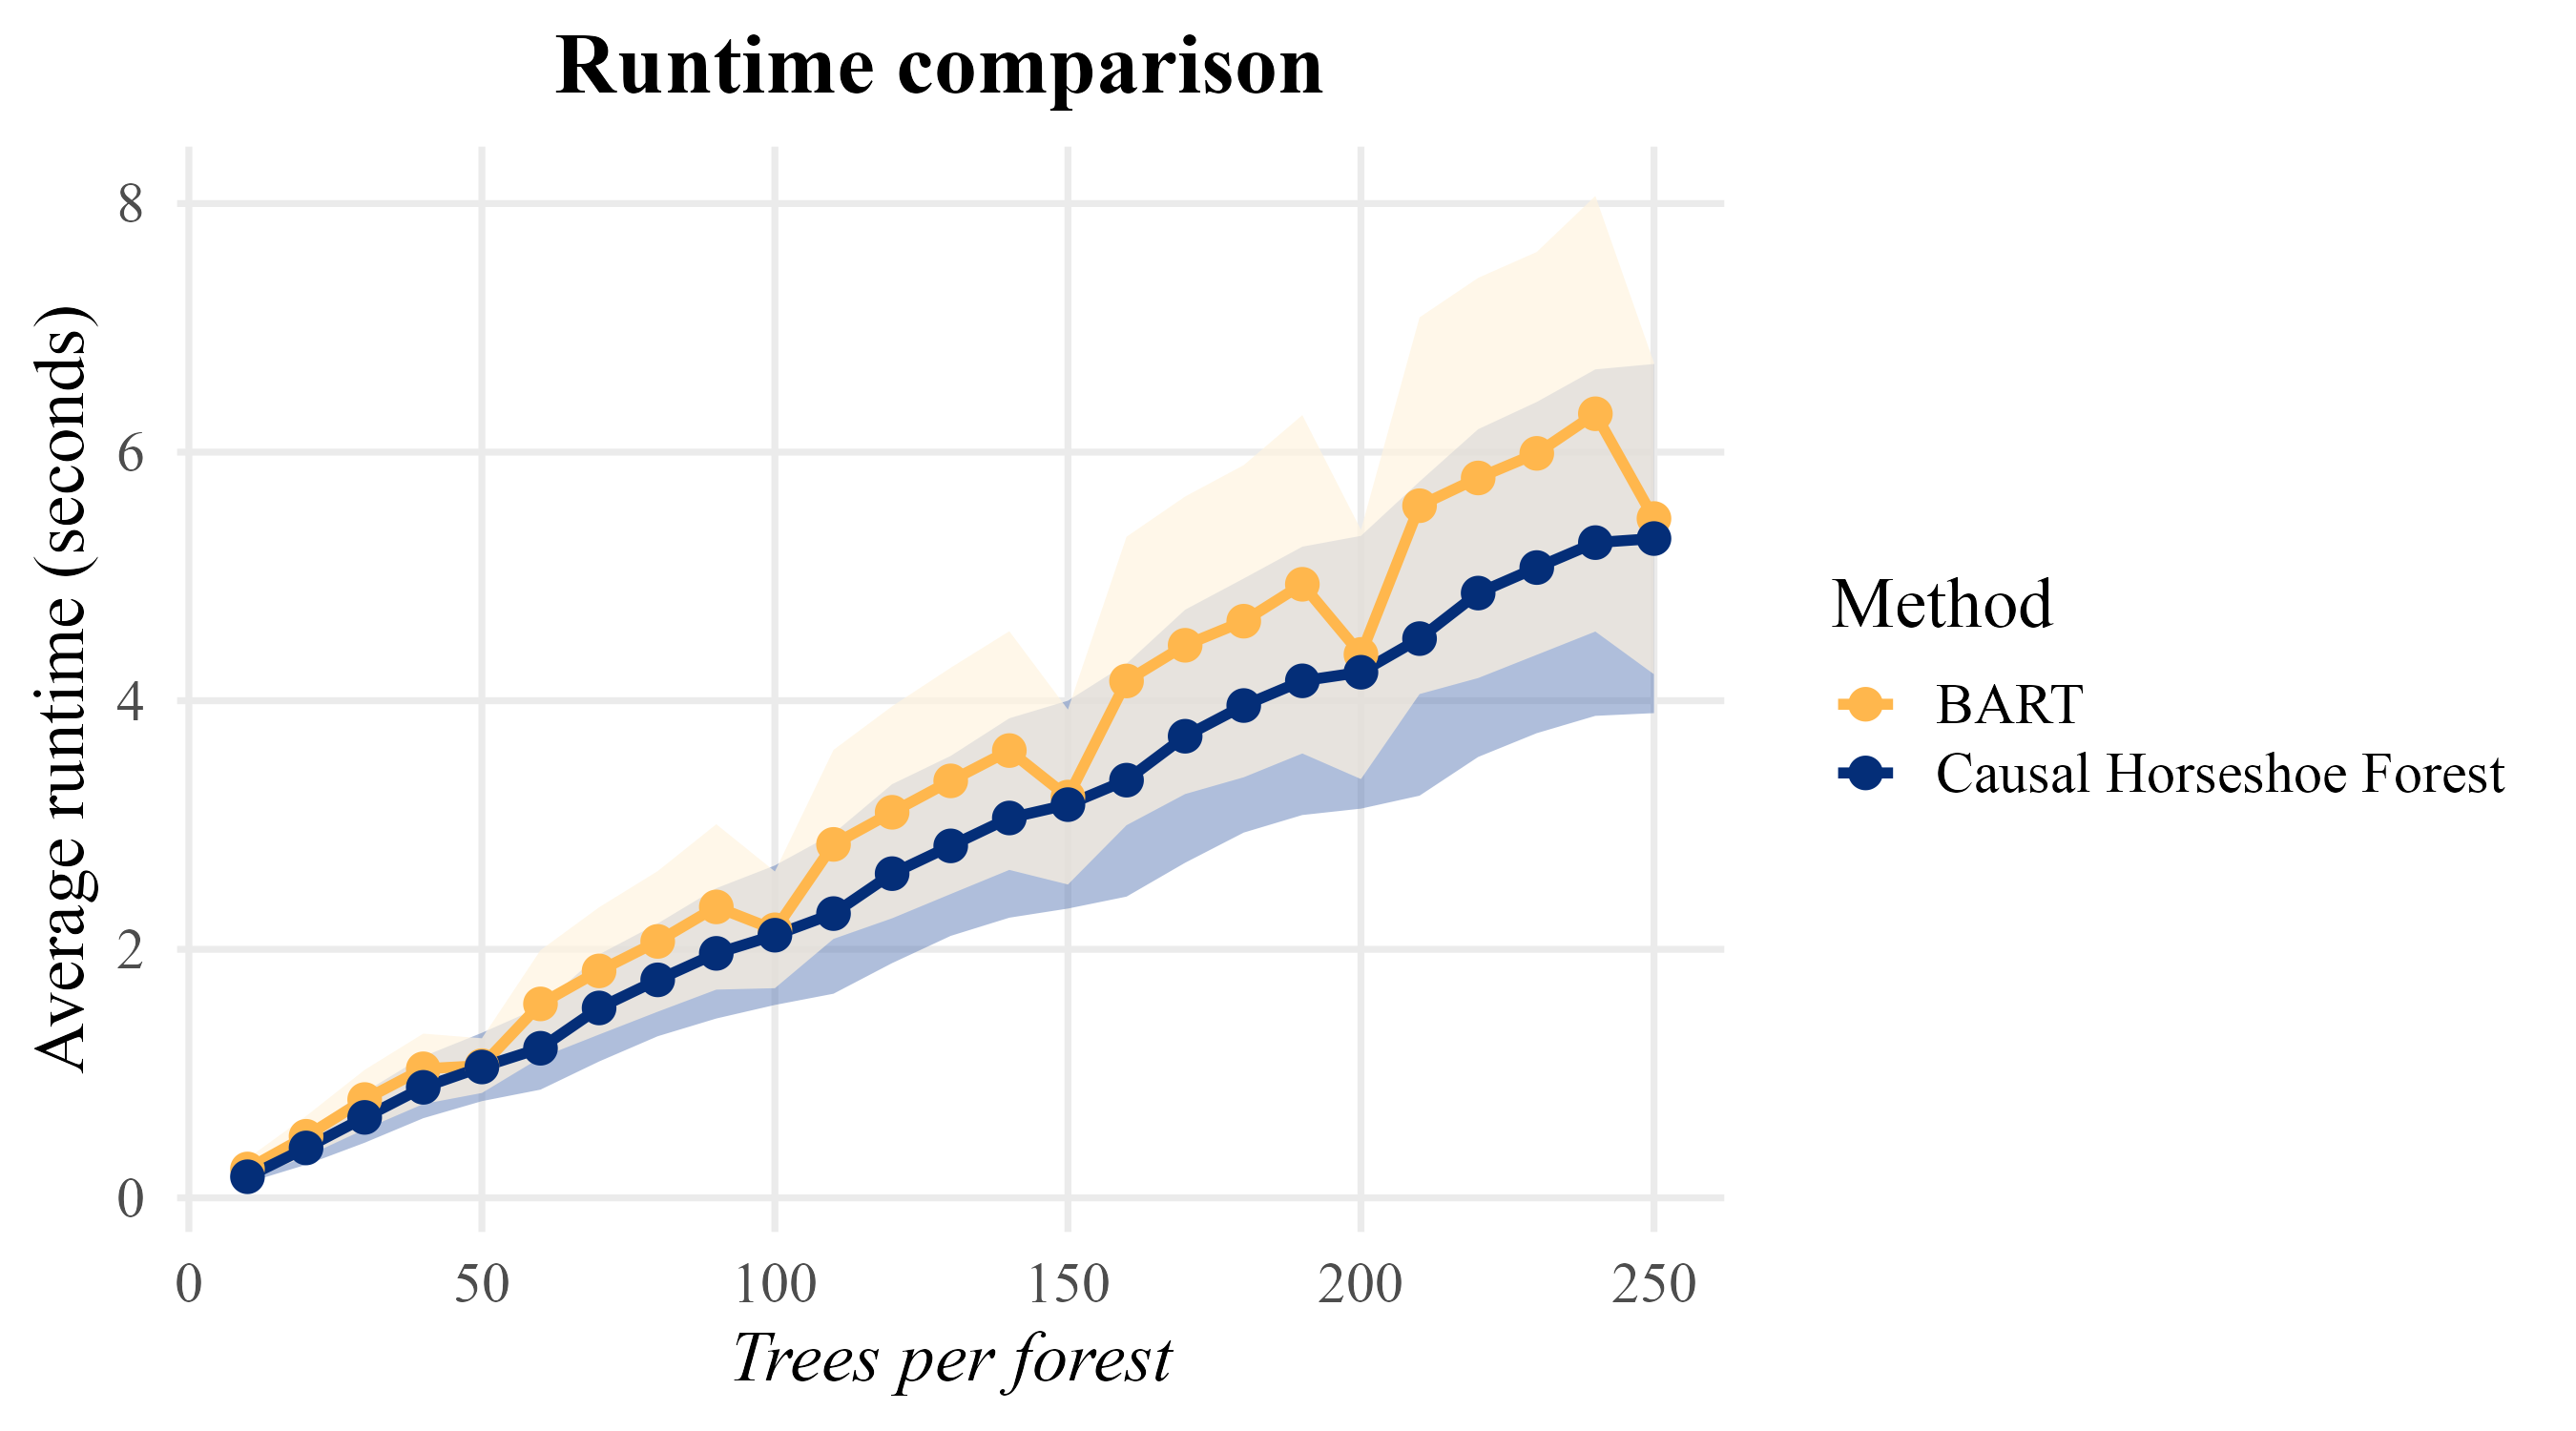
\includegraphics[width=\linewidth]{runtime_comparison_BART_vs_CHF.png}
  \caption{
    Average wall-clock runtime as a function of the number of trees per forest ($m$), averaged over five data-generating processes with 200 repetitions per setting. Shaded bands represent $\pm$ one standard deviation.
  }
  \label{fig:runtime}
\end{figure}


We conducted an empirical runtime comparison between Bayesian Additive Regression Trees (BART) \citep{bartRpackage} and the proposed Causal Horseshoe Forest (CHF) under uncensored data-generating processes.
Five distinct data-generating processes were considered, varying in sample size and covariate dimension.
Both methods were run under identical configurations, and wall-clock runtime was recorded in seconds.
This procedure was repeated 200 times per setting, resulting in a total of 1000 runs.
For the Causal Horseshoe Forest, we fixed the number of trees to $m$ per forest, yielding $2m$ trees in total across the treatment and control forests.
For BART, the ensemble size was fixed to $2m$ trees to ensure a comparable total number of trees across methods. Figure~\ref{fig:runtime} reports the average runtime as a function of $m$,
aggregated across data-generating processes and repetitions, with variability
summarised by one standard deviation.
Across the range of ensemble sizes considered, the two methods exhibit very
similar scaling behaviour.
In this implementation, CHF is marginally faster on average, which we attribute to implementation-level optimisations rather than fundamental algorithmic differences.
Overall, these results indicate that CHF achieves computational performance comparable to BART while offering additional modelling flexibility through explicit shrinkage priors.
